\documentclass[11pt]{article}
\usepackage{acl}
\usepackage{times}
\usepackage{latexsym}
\usepackage[T1]{fontenc}
\usepackage[utf8]{inputenc}
\usepackage{microtype}
\usepackage{inconsolata}
\usepackage{booktabs}
\usepackage{amsmath}
\usepackage{graphicx}
\usepackage{xcolor}

\title{Who Taught This Model? Prompt-Conditioned Contrastive Attribution for Public Teacher-Student Language Models}

\author{
Luiz Venosa \\
Bocconi University \\
\texttt{luiz.lima@studbocconi.it}
}

\begin{document}
\maketitle

\begin{abstract}
Model distillation transfers behavior from a larger teacher model to a smaller student model, but the teacher behind a released student is not always verifiable from the model card alone.
Recent work asks whether a student model's teacher can be inferred from its outputs.
I study a practical version of this problem using public teacher-student language-model pairs with documented lineage.
For each prompt, I generate responses from all candidate teachers and from the corresponding public student, then train a prompt-conditioned contrastive encoder that pulls a student response toward its documented teacher response and away from other same-prompt teacher responses.
On a four-way public-lineage attribution task, the best completed MiniLM encoder reaches 60.44\% single-prompt accuracy and 82.84\% top-2 accuracy, compared with a 25\% chance baseline.
When predictions are aggregated across multiple prompts, accuracy rises sharply, reaching 90.0\% with four prompts and 97.5\% with eight.
These results suggest that public student models preserve detectable teacher-specific fingerprints, but also show that attribution remains sensitive to task type, model family overlap, and training stability.
\end{abstract}

\section{Introduction}

Distillation is a common way to transfer capabilities from a large teacher language model into a smaller student.
This practice improves efficiency, but it also raises a provenance question: \textbf{given only a student model's outputs, can we infer which teacher influenced it?}
Reliable teacher attribution would be useful for transparency, auditing, and understanding how behavioral patterns survive distillation.

The starting point for this project is \citet{wadhwa-etal-2025-taught}, who study teacher tracing in a controlled distillation setup.
They train students on teacher-generated data and show that teacher identity can sometimes be recovered from student outputs.
My project adapts this question to a messier but realistic setting: instead of training all students from scratch, I use public teacher-student model pairs whose model cards document a teacher or source model.

This public-lineage setting changes the problem.
The labels are more realistic, but less controlled: model cards vary in detail, some students inherit from a family rather than one clean teacher, and public checkpoints may include additional instruction tuning.
To reduce topic leakage, all candidate teachers and students answer the same prompt bank.
The resulting example contains one student response, several same-prompt teacher responses, and the documented teacher label.

I make three contributions.
First, I build a reproducible pipeline for public teacher attribution from prompt generation to contrastive evaluation.
Second, I introduce a prompt-conditioned contrastive encoder that compares each student response with same-prompt candidate teacher responses.
Third, I evaluate the method on single-prompt and set-level attribution, showing that individual responses are noisy but teacher fingerprints become much clearer when aggregating responses across prompts.

\section{Experiments}

\subsection{Teacher-Student Pairs}

The main experiment uses four public teacher-student lineages (Table~\ref{tab:pairs}).
Two pairs have strong explicit model-card evidence, while the two FLAN-T5 pairs are treated as medium-confidence same-family instruction-distilled lineages.
The task is therefore four-way classification, with chance accuracy of 25\%.

\begin{table}[t]
\centering
\small
\begin{tabular}{lll}
\toprule
Teacher ID & Teacher & Student \\
\midrule
\texttt{gpt2} & \texttt{gpt2} & \texttt{distilgpt2} \\
\texttt{qwen15\_18b} & Qwen1.5-1.8B & MiniPLM-Qwen-200M \\
\texttt{flan\_t5\_base} & FLAN-T5-base & LaMini-FLAN-T5-248M \\
\texttt{flan\_t5\_small} & FLAN-T5-small & LaMini-FLAN-T5-77M \\
\bottomrule
\end{tabular}
\caption{Default public teacher-student pairs. The experiment uses documented public lineages rather than training new students from scratch.}
\label{tab:pairs}
\end{table}

\subsection{Prompt Bank and Data}

The prompt bank follows the broad task mix of \citet{wadhwa-etal-2025-taught}: summarization, question answering, and instruction following.
I use prompts from CNN/DailyMail, SumpubMed, Rotten Tomatoes, CommonsenseQA, OpenBookQA, QuaRel, and Alpaca-style instructions.
All four teachers and all four public students answer the same prompts.

The completed run produced 3,000 test prompts and 29,742 training prompts after filtering and dataset availability.
For each prompt, the attribution row stores the prompt, one student response, all candidate teacher responses, the true teacher ID, task metadata, and source-dataset metadata.
The test file contains 12,000 attribution rows, corresponding to 3,000 prompts times four student labels.

\subsection{Contrastive Attribution Model}

Each input to the encoder is a prompt-response pair:
\begin{equation}
z = f_{\theta}(x, y),
\end{equation}
where $x$ is the prompt and $y$ is either a student response or a teacher response.
The encoder is shared for students and teachers.
The main completed model uses \texttt{sentence-transformers/all-MiniLM-L6-v2} with a projection head and a teacher-classification head.

For each row, the student embedding is the anchor, the documented teacher response is the positive, and the other teacher responses to the same prompt are negatives.
The contrastive part of the loss is:
\begin{equation}
\mathcal{L}_{\mathrm{NCE}} =
-\log \frac{\exp(\mathrm{sim}(z_s,z_{t^+})/\tau)}
{\sum_{k}\exp(\mathrm{sim}(z_s,z_{t_k})/\tau)} ,
\end{equation}
where $\mathrm{sim}$ is cosine similarity and $\tau$ is the temperature.
The final objective adds a supervised teacher-classification term:
\begin{equation}
\mathcal{L} = \mathcal{L}_{\mathrm{NCE}} + \lambda \mathcal{L}_{\mathrm{CE}} .
\end{equation}

\subsection{Baselines and Metrics}

The final baseline script implements four WTYT-style text baselines: Bag-of-Words same-prompt similarity, BERTScore same-prompt similarity \citep{zhang2020bertscore}, Bag-of-Words logistic regression, and 1--4 gram logistic regression.
The POS-template baseline from \citet{wadhwa-etal-2025-taught} is not used in the final comparison because I could not reliably reproduce it in the environment.

I report top-1 accuracy, top-2 accuracy, one-vs-rest ROC-AUC, confusion matrices, task breakdowns, dataset breakdowns, and set-level accuracy.
Set-level attribution averages embeddings over multiple prompts before comparing the student fingerprint to teacher fingerprints.

\section{Results}

\subsection{Single-Prompt Attribution}

Table~\ref{tab:main} shows the current main contrastive result and WTYT-style baselines.
The MiniLM contrastive model reaches 60.44\% accuracy and 82.84\% top-2 accuracy on 12,000 test rows.
This is well above the 25\% chance baseline, showing that public students preserve detectable teacher-specific signals.
The strongest single-prompt baseline is the 1--4 gram logistic classifier, which slightly outperforms the contrastive encoder in top-1 accuracy.
The contrastive encoder is therefore best understood as a teacher-space representation model rather than as a replacement for every lexical classifier.

\begin{table}[t]
\centering
\small
\begin{tabular}{lccc}
\toprule
Method & Acc. & Top-2 & AUC \\
\midrule
BoW same-prompt & 32.83 & 58.63 & 54.82 \\
BERTScore same-prompt & -- & -- & -- \\
BoW classifier & 58.36 & 87.58 & 81.89 \\
1--4 gram classifier & \textbf{62.17} & \textbf{88.14} & \textbf{83.89} \\
\midrule
MiniLM contrastive & 60.44 & 82.84 & 68.14 \\
\bottomrule
\end{tabular}
\caption{Test results on the four-way public-lineage attribution task. BERTScore failed in the final baseline run and is left unreported.}
\label{tab:main}
\end{table}

Performance varies strongly by task.
The model is best on question answering, where it reaches 84.18\% accuracy.
Instruction following is more difficult at 60.90\%, and summarization is hardest at 44.47\%.
This suggests that some tasks expose teacher-specific answer habits more clearly than others.
Summarization may compress outputs into more similar forms, making lineage harder to detect from a single example.

\subsection{Set-Level Attribution}

Teacher attribution becomes much easier when multiple prompts are aggregated, as shown in the set-level plot below.
With two prompts, accuracy rises to 73.75\%; with four prompts, to 90.0\%; and with eight prompts, to 97.5\%.
At 16 or more prompts, the sampled set-level evaluation reaches 100\%.
This is the clearest evidence for the project hypothesis: a single response can be noisy, but a student model exhibits a more stable teacher fingerprint across prompts.

\begin{center}
\centering
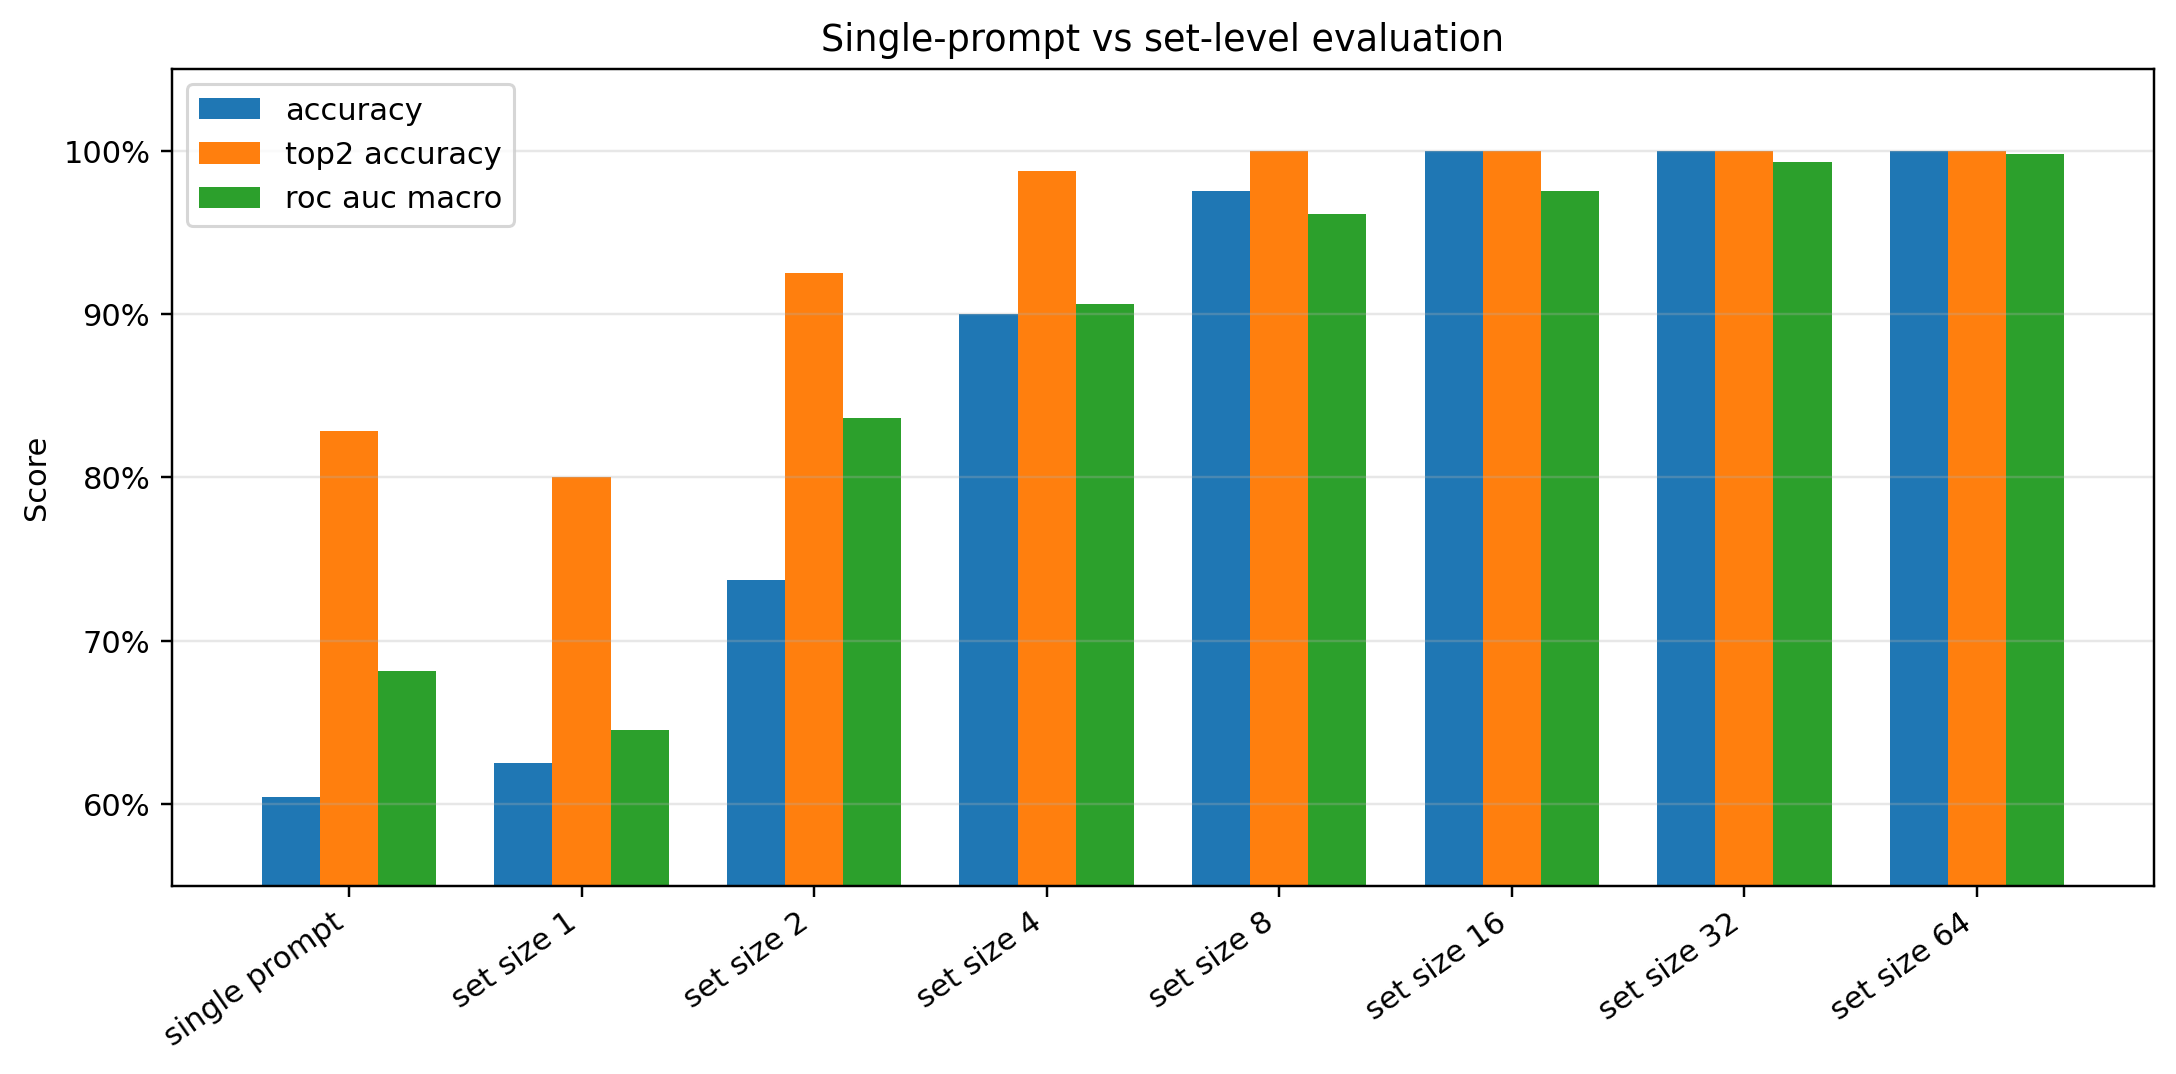
\includegraphics[width=\columnwidth]{figures/11_single_vs_set_level_comparison.png}
{\small \textbf{Figure 1:} Single-prompt versus set-level evaluation. Aggregating multiple prompts sharply improves teacher attribution accuracy and AUC.}
\end{center}

\subsection{Ablations and Larger Encoders}

I ran seven fixed five-epoch MiniLM ablations over temperature, classification weight, learning rate, and projection dimension.
The best ablation by test accuracy was a higher learning rate run (\texttt{lr5e5}) at 60.08\%, but it did not beat the full early-stopped MiniLM model.
The best validation ablation used a larger projection dimension, but reached only 59.68\% on test.
Overall, the ablations indicate that performance is not mainly limited by these shallow hyperparameters.
The training curve below also shows why I selected the early-stopped checkpoint: loss continues to fall, but validation accuracy flattens around 60--61\%, suggesting increasing specialization without clear attribution gains.

\begin{center}
\centering
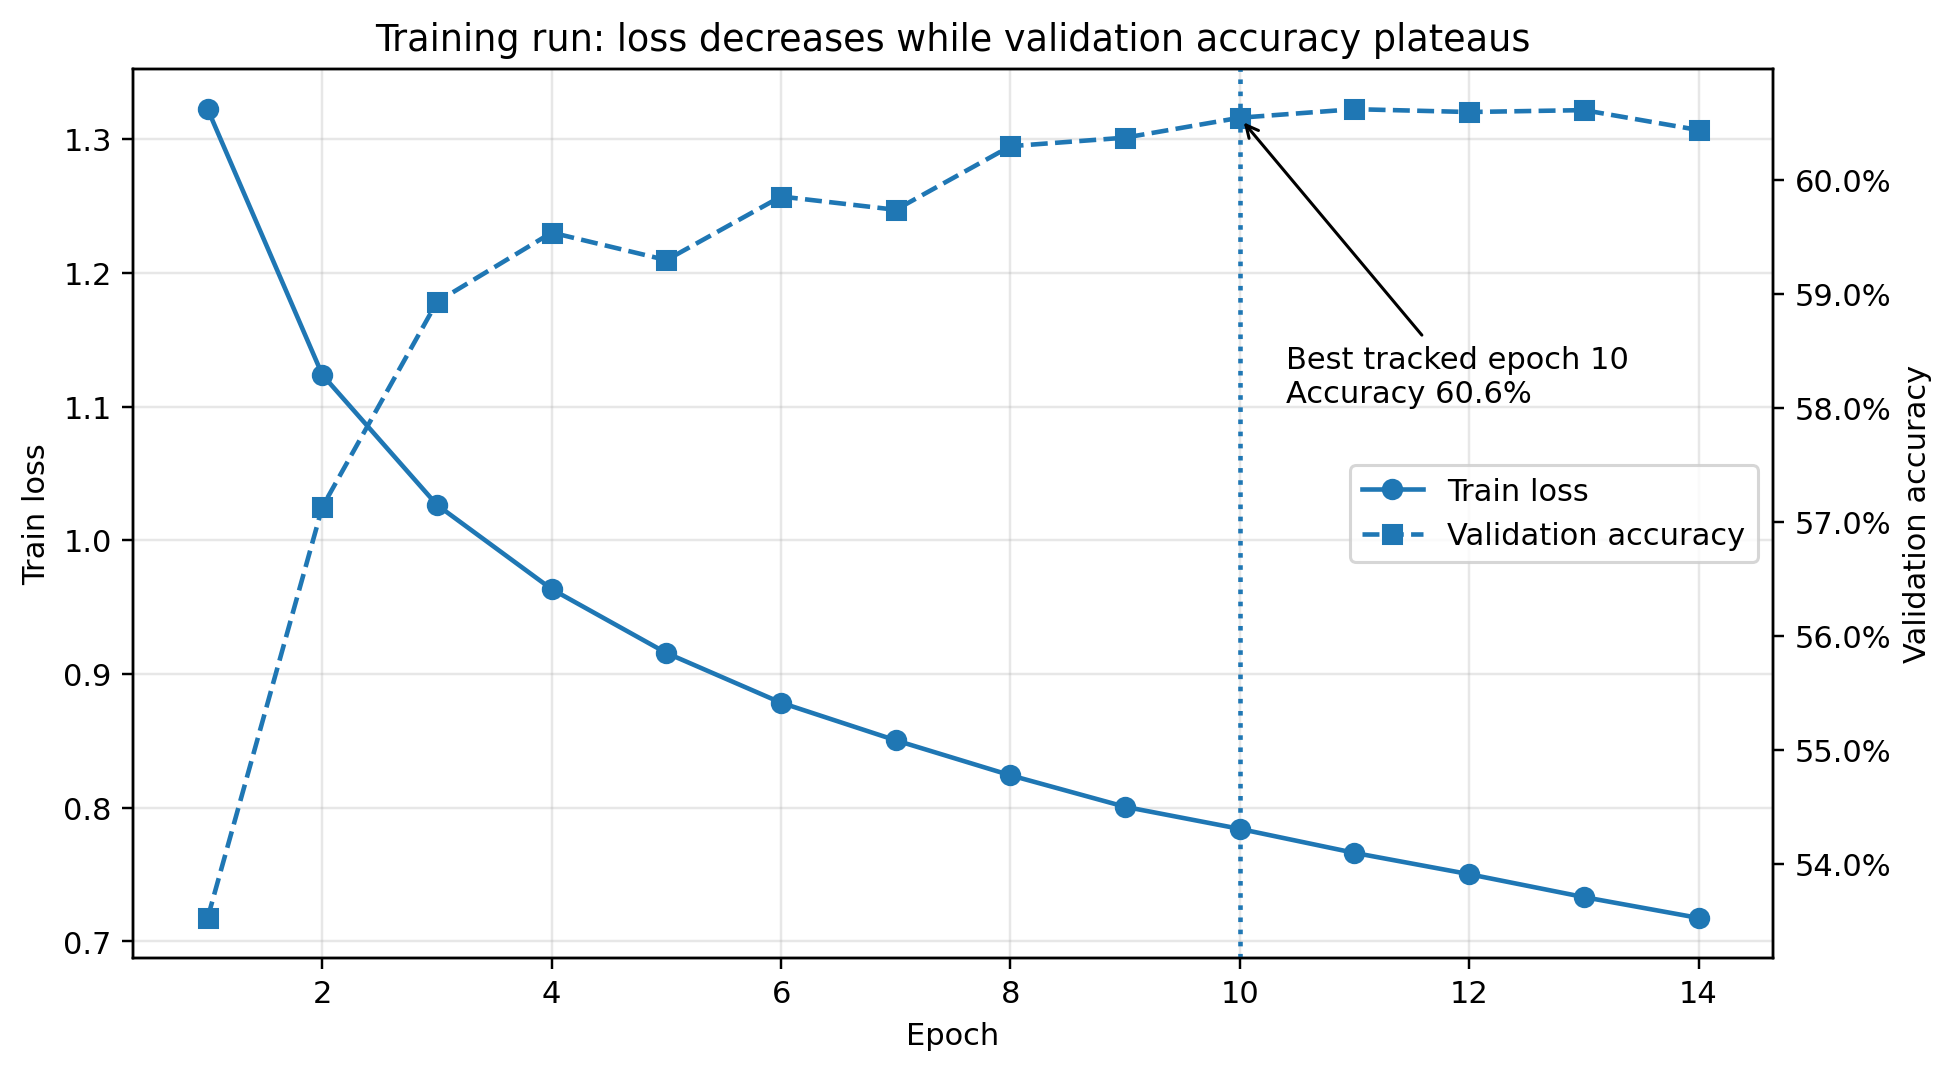
\includegraphics[width=\columnwidth]{figures/01_training_loss_accuracy.png}
{\small \textbf{Figure 2:} Training loss decreases steadily while validation accuracy plateaus, motivating early stopping rather than longer training.}
\end{center}

I also explored larger encoders.
E5-large improved for three epochs but collapsed to chance accuracy at epoch 4, suggesting unstable full fine-tuning.
DeBERTa-v3-base produced NaN losses under the available mixed-precision setup.
Because of time constraints, I treat these as preliminary failed scaling attempts rather than final comparisons.
They indicate that larger backbones may require lower learning rates, bf16 precision, freezing schedules, or style-specific pretraining before they help this task.

\section{Related Work}

This project is most directly inspired by \citet{wadhwa-etal-2025-taught}, who introduce teacher tracing in model distillation.
They study controlled task distillation and show that lexical features alone are unreliable, while syntactic templates can preserve teacher footprints.
My work keeps the teacher-attribution question but replaces controlled student training with documented public lineages and adds a contrastive same-prompt encoder.

The contrastive component is related to InfoNCE and supervised contrastive learning \citep{oord2018representation,khosla2020supervised}.
It is also motivated by authorship attribution work.
\citet{ai-etal-2022-whodunit} show that contrastive fine-tuning of pretrained encoders can learn author-specific representations.
\citet{huertas2024isolating} argue that authorship models must separate style from content, which is closely related to this project: teacher attribution should capture response style and behavior rather than prompt topic.

\section{Conclusion}

I built and evaluated a public-lineage teacher attribution pipeline for language models.
The main completed contrastive MiniLM model achieves 60.44\% single-prompt accuracy and 82.84\% top-2 accuracy on a four-way attribution task, and set-level aggregation reaches much higher performance.
The results support the idea that student outputs preserve teacher-specific fingerprints, especially when evidence is collected across prompts.
At the same time, task breakdowns and failed larger-encoder attempts show that teacher attribution is not solved by scale alone.
Future work should add more verified lineages, stabilize larger or style-specific encoders, and test harder cross-dataset and paraphrased-prompt settings.

\section*{Limitations}

This project uses public model-card lineages rather than controlled distillation, so labels are realistic but noisier than in a laboratory setup.
The four-way label space is small, and two classes are closely related FLAN-T5-family models.
The same-prompt setting assumes candidate teacher responses are available for the prompts being evaluated.
Generation settings may also affect attribution because decoding style can change surface behavior.
Finally, larger encoder experiments were not completed successfully: E5-large collapsed after early improvement, and DeBERTa-v3-base produced NaN losses under the first training configuration.
These failures are informative, but they should not be interpreted as final evidence against larger encoders.

\section*{Acknowledgments}

I thank the Language Technology course staff for guidance on project design and report structure.

\bibliography{references}

\end{document}
